\documentclass{ULBreport}
\usepackage{comment}
\usepackage{fontspec}
\setmainfont{Arial} 

\sceau{Pictures/sceauULB.jpg}

\addbibresource{biblio.bib}

\begin{document}

\titleULB{
	title={Application: déclaration et demande de subsides des camps de mouvement de jeunesse auprès de l'Office de la Naissance et de l'Enfance (ONE)},
	studies={2021-2022},
	course={STIC-B505 - Conception et gestion de banques de données},
	author={David MANFROY\\Selim BEN ISMAIL},
	date={Année académique 2021-2022},
	teacher={Frédéric SERVAIS\\Manon LEGRAND},
	logo={Pictures/logo_mastic_long_petit.png},
	manyAuthor
}

%----- Introduction  ---------
\chapter{Introduction}
\section{Domaine d'application}
	Chaque année, les unités de cinq fédérations de mouvements de jeunesse organisent des camps pour les plus jeunes. Ces camps sont situés généralement dans des provinces reculées de Belgique, mais pas seulement. En effet, nous retrouvons également des camps à la côté, à l'étranger, etc. 
	Ces unités sont agréés par l'Office de la Naissance et de l'Enfance. Dans ce cadre, ils peuvent demander des subsides pour chaque camp organisés qui respectent les normes d'encadrement en vigueur. Pour se faire, les unités doivent remplir les formalités administratives suivantes: 1/ déclarer le camp préalablement et 2/ introduire une demande de subsides. Ces démarches administratives sont remplies par les unités au moyen de formulaires envoyés à l'ONE. 


\subsection{Fédération de mouvement de jeunesse}\label{fmj}
En Belgique, les fédérations de mouvement de jeunesse sont: \begin{itemize}
	    \item Les Scouts;
	    \item Les Guides de Belgique;
	    \item Les Patros;
	    \item Les Guides et Scouts pluralistes;
	    \item Les Faucons Rouges.
	\end{itemize}
Chaque unité est liée à une \textbf{seule fédération bien précise}. 


\subsubsection{Une même adresse, pour plusieurs unités de différentes fédérations}
Mais il n'est pas rare de retrouver plusieurs unités de différentes fédération à un endroit octroyé par la commune. Bien souvent, nous retrouvons une unité Guide avec une unité Scout dans les mêmes locaux communaux. Une même adresse peut donc être partagée par plusieurs unités.

\subsubsection{Un gestionnaire de dossier ONE par fédération}
Il y a un gestionnaire de dossier par fédération. Un même agent va traiter toutes les demandes de subsides qui émanent des unités Patros par exemple.



\subsection{Unité de mouvement de jeunesse}
Chaque unité est divisée en \textbf{section }qui accueille chacune enfant de tranche d'âge différent. Par exemple: chez les Guides, le section qui accueille les plus petits sont les nutons (5 - 6 ans), puis les lutins (7 - 11 ans), puis les guides aventures(11 - 15 ans), et enfin guide horizon (15-17 ans). 

Les autres fédérations ont également une subdivision qui ressemble à celle des Guides pour leur unité. Les appellations diffèrent juste d'une fédération à l'autre, mais la logique d'accueil par tranche d'âge est identique. 

\subsubsection{Un camp par section}
Chaque section part en camp dans différents endroits; l'unité organise donc un ou plusieurs camps (une par section plus ou moins). Il peut arriver également qu'un même lieu de camp accueillent plusieurs sections, quelle que soit l'unité. 


	
\section{Le Projet}
Le projet proposé dans ce travail est de développer une application qui transforme les formulaires papiers en formulaire à compléter en ligne. 


\subsection{Explication du processus administratif}
Le processus administratif actuel est le suivant: 
\begin{enumerate}
    \item L'unité envoie à l'ONE les formulaires de déclaration d'activité de ses différentes sections (avant le 30 avril de l'année).
    \item L'administration centrale de l'ONE réceptionne les déclarations d'activités et les inventorie dans la base de données. 
    \item Une fois toutes les déclarations encodées, les camps sont triés en fonction des provinces. L'administration centrale envoie ensuite à ses subrégions la liste des camps les concernant.
    \item Les administrations subrégionales attribuent chaque camp à une coordinatrice accueil.
    \item Une fois le camp passée, les sections remplissent les formulaires de demandes de subsides et les transmettent à l'unité. Après vérification, l'unité envoie les formulaires à l'ONE avant le 30 septembre.
    \item L'ONE et l'agent traitant analyse la demande de subsides et vérifie les normes d'encadrement (voir point suivant \ref{subside_camp_explications}. Dans les fait, les agents proposent des décisions qui sont ensuite validé par l'Administrateur général de l'ONE. 
    \item Une décision de subvention est prise par l'ONE et l'unité reçoit le paiement du subside.
    \item La décision est envoyée au(x) Responsables d'unité. 
\end{enumerate}


\subsection{Subsides des camps: explications}\label{subside_camp_explications}
Les camps peuvent prétendre à des subsides de la Communauté française. Ce subside est payé par l'ONE qui vérifie au préalable si les normes minimales d'encadrement sont respectées durant le camp. 

\subsubsection{Normes d'encadrement (quantité)}
Les normes d'encadrement sont décrits dans le décret centres de vacances de la Communauté française. Ces normes sont les suivantes: 

\begin{itemize}
    \item 1 animateur par groupe de 8 enfants de moins de 6 ans
    \item 1 animateur par groupe de 12 enfants de plus de 6 ans.
    
    
\end{itemize}

\subsubsection{Normes d'encadrement (qualité)}
Outre le nombre d'animateurs, il faut également respecter des normes de qualité de l'équipe d'encadrement: 1 animateur sur trois doit être porteur du brevet d'animateur centres de vacances. Le brevet est délivré par des organismes de formation agréé. 

Le camp doit également être coordonnée par un responsable qualifié (un animateur porteur a minima du brevet d'animateur ayant une année d'expérience ou être porteur d'un brevet de coordinateur de centres de vacances).

\subsubsection{Décision de la demande de subsides}
La demande de subside peut faire l'objet de plusieurs décisions de la part de l'administration: 

\begin{itemize}
    \item Soit la décision est favorable car les critères d'encadrement et de qualité de l'animation sont remplies,
    \item soit favorable partiellement car le critère d'encadrement n'est pas tout à fait respecté mais la qualité d'animation rattrape la lacune,
    \item soit défavorable car les normes d'encadrement ne sont pas du tout respectées. 
\end{itemize}



%\subsection{Informatisation du processus de déclaration et de demandes de subsides des camps}
%Le Projet consistera à traduire ce processus administratif de déclaration et demande de subsides pour les camps. Voici les spécificités à prendre en compte pour ce projet:
%\begin{itemize}
 %   \item Les différentes fédérations de mouvement de jeunesse; chaque unité dépends d'une fédération de mouvement de jeunesse. Cette dernière centralise également la gestion logistique et administratives des camps de ses membres. Mais elle ne gère pas les demandes de subventions de ses unités. 
  %  \item La structure unité, section; en effet, l'ONE donne l'agrément à la fédération. Les unités et les sections reçoivent par héritage l'agrément (pour pouvoir prétendre aux subsides), mais c'est bien l'unité qui est reconnu comme pouvoir organisateur (et non pas la section). Il est donc logique que ce soit l'unité qui reçoive les rapports de visite et les subventions de ses sections.
   % \item L'aspect d'administration centrale et régionale propre à l'ONE; la centrale réceptionne et traite les formulaires, mais les visites d'accompagnement de terrain sont confiées aux subrégions.  
    
% (partie supprimée suite à réunion d'accompagnement)   \item Les visites d'accompagnement; vu la quantité très importante d'activité de camp, il est impossible de faire une visite systématique. Ainsi, chaque unité voit l'un de ses camps visités au moins une fois tous les trois/quatre ans. Il y a donc un historique des visites effectués. 
%\end{itemize}	
	

%\section{Identification des utilisateurs cibles du système}

%\subsection{L'Office de la Naissance et de l'Enfance (ONE)}

%\subsubsection{Décision concernant la demande de subsides}





\section{Utilisation du Projet}
\subsection{Explications}
Considérant le processus et les spécificités décrite supra, nous allons concevoir une application qui reprend la plupart des champs des divers formulaires de déclaration d'activité et de demande de subsides\footnote{Ces formulaires sont disponibles sur le site \url{http://www.centres-de-vacances.be} de l'ONE}. 



%\subsubsection{Vue sur les camps:} la base de données ainsi constituée servira à lister les camps par province en vue d'une visite de terrain par les subrégions; pour faciliter également l'organisation des visites, nous allons mettre en relation les unités qui n'ont pas été visités dans les quatre dernière année. Une unité rentrera donc dans la catégorie "visite prioritaire" dans le cas où aucune de ses sections n'a été visité dans les quatre années passées. 

%   supprimé suite à réunion d'accompagnement 
%\subsubsection{Assignation des camps à une coordinatrice} 
%Nous prévoirons également une assignation à une coordinatrice en particulier (assignation automatique ou manuelle). Cela permettra à une coordinatrice accueil de lister les camps qu'elle doit visiter et les camps prioritaires. Une case visite effectuée sera ajoutée afin d'encoder la visite. Et différent champs permettront de renseigner le résultat de la visite. 


\subsection{Utilisateurs cibles de l'application}

\subsubsection{Le responsable d'Unité} Il réceptionne tous les courriers officiels et gère l'aspect administratif. C'est cette personne qui déclare et qui réalise les demandes de subsides sur la plateforme. Elle reçoit également les notifications de décision concernant les demandes de subsides. 

%partie supprimé suite à visite d'accompagnement
%\subsubsection{La Coordinatrice accueil} reçoit quelques camps dans ses attributions pour effectuer des visites de terrain. Elle rédige un rapport de visite qu'elle transmet au Responsable d'unité, mais également à l'agent traitant. 

\subsubsection{L'Agent traitant ONE}
L'agent analyse et traite les demandes de subsides rentrées. Il y a un agent ONE qui s'occupe des dossiers d'une fédérations précise. Il y a donc 5 agents traitant. 

\subsection{Cas d'utilisation de la plateforme}

\subsubsection{Création et modification des unités}
L'application doit permettre de créer les unités de mouvement de jeunesse et de les relier à une fédération de mouvement de jeunesse. Les ajouts de ces données sont uniquement réalisés par l'ONE qui vérifie si ces unités existent et si elles sont agréées pour organiser des camps. 

Dans le cadre de ce projet, Cette partie de l'application se fera via l'application phpMyAdmin. 


\subsubsection{Mise à jour du Responsable d'unité}
L'application permettra de mettre à jour le responsable d'unité. Un bouton dédié à la mise à jour de l'identité, des coordonnées de contact. 



\subsubsection{Déclaration des camps}
Un des écrans sera destiné à la déclaration d"activité qui servira à récolter les données de camp. Les données renseignées permettront de réaliser le traitement des normes d'encadrement. 
La déclaration permettra d'ajouter les enfants et les encadrants pour chaque camp. 

\subsubsection{Demande de subsides des camps déclarés}
Un autre écran permettra de compléter et d'envoyer la demande de subsides.


\subsubsection{Décision de subsides (par l'ONE)}
Un champs de décision de subsides sera également présent. Plusieurs items constitueront la partie décision (justification, sommes de subsides, raison du refus, etc.)









%----- Schéma Entité-Relation ---------
\chapter{Schéma conceptuel (entité-association)}
\section{Le schéma}
\begin{figure}[H]
    \centering
    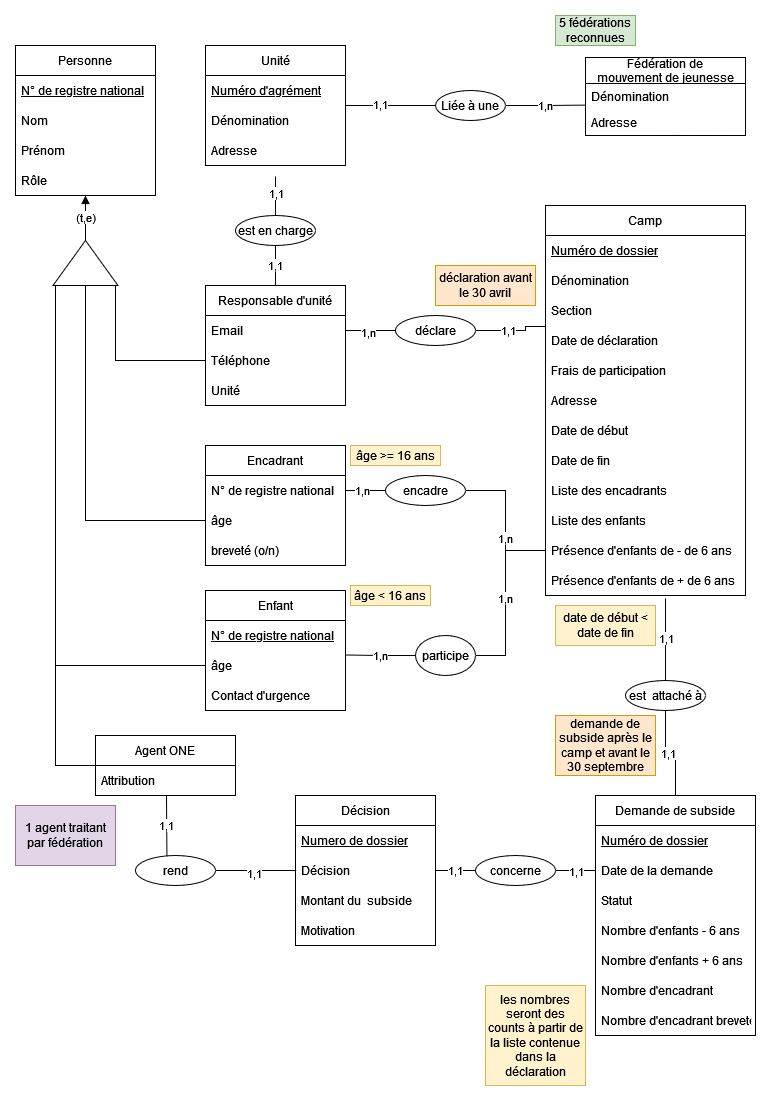
\includegraphics[height=15cm]{Pictures/modele_ea.jpg}
    \caption{Modèle entités-associations}
    \label{fig:modele_ea}
\end{figure}

\subsection{Les entités: quelques explications}

\subsubsection{Fédération de mouvement de jeunesse}
Il n'existe que cinq fédérations de mouvement de jeunesse (cf. point \ref{fmj}). 

\subsubsection{Unités}
Chaque unité appartient à une seule fédération de mouvement de jeunesse. Il y a également plusieurs sections au sein d'une unité, mais la modélisation n'est pas pertinente pour notre domaine d'application. Une unité organise plusieurs camps; une par section environs. L'information de section figure dans l'entité camp. 


\subsubsection{Correspondant: chef d'unité}
Il s'agit de la personne de contact de l'unité. L'adresse de correspondance est parfois différente de celui du Pouvoir organisateur (qui est l'adresse officielle). Une adresse mail et un numéro de téléphone est également demandé. 

\subsubsection{Déclaration de camp}
Le chef d'unité déclare le:
\begin{itemize}
    \item \textbf{nom du camp}: il s'agit parfois du thème du camp ou du lieu-dit (une prairie, un endroit proche d'une rivière, etc.)
    \item \textbf{l'adresse} de ce camp
    \item quelques \textbf{caractéristiques d'accueil}, comme par exemple la tranche d'âge accueillie, les frais de participations demandées aux parents, etc.
    \item les \textbf{dates du camp}
    \item et enfin une \textbf{liste des encadrants chef} et une liste \textbf{des animés enfants}.
\end{itemize}

La déclaration doit parvenir à l'ONE avant le 30 avril. L'ONE envoie ensuite un formulaire de demande de subsides avec le numéro du dossier du camp.

Le chef déclare les camps au nom de l'unité qui les organise. Les déclarations sont donc liées à l'unité dans notre base de données. Une unité organise un ou plusieurs camps généralement en fonction du nombre de ses sections. 


% supprimé 
%\subsection{Le responsable qualifié}
%Le responsable qualifié sera la personne de contact et physiquement sur place pour les visites des coordinatrices accueil. Il fait parti du personnel d'encadrement du camp et n'est pas nécessairement le correspondant de l'unité.


\subsubsection{La demande de subsides}
La demande de subsides intervient après le déroulement du camp d'été et doit être envoyé avant le 30 septembre. 

Les données demandées sont le nombre d'enfants et de chefs par jour, l'identité et la caractéristique des enfants (âge, porteur de handicap, en situation défavorisée, etc.) et des chefs (âge, breveté). 

La demande de subsides est liée directement à la déclaration et est traité par un agent traitant qui rend une décision. 

\subsubsection{Agent traitant ONE}
Il y a un agent traitant par dossier de fédération. Un même agent s'occupe donc de l'ensemble des dossiers Patros, un autre des dossiers Guides, etc. 


\subsubsection{Décision concernant la demande de subsides}
La demande de subsides débouche sur une décision de la part de l'ONE (agent traitant). En fonction de la décision, une somme de subsides est accordée pour le camp.


\subsection{Héritage is-a}

\subsubsection{Personne}
Dans le schéma conceptuel, les responsables d'unité, les enfants, animateurs et agent ONE sont des personnes. Un super-entité Personne rassemble les informations d'identification personnelle. 


%---- Schéma Schéma logique relationnel -------
\chapter{Schéma Logique Relationnel}
\section{Le schéma}
\begin{figure}[H]
    \centering
    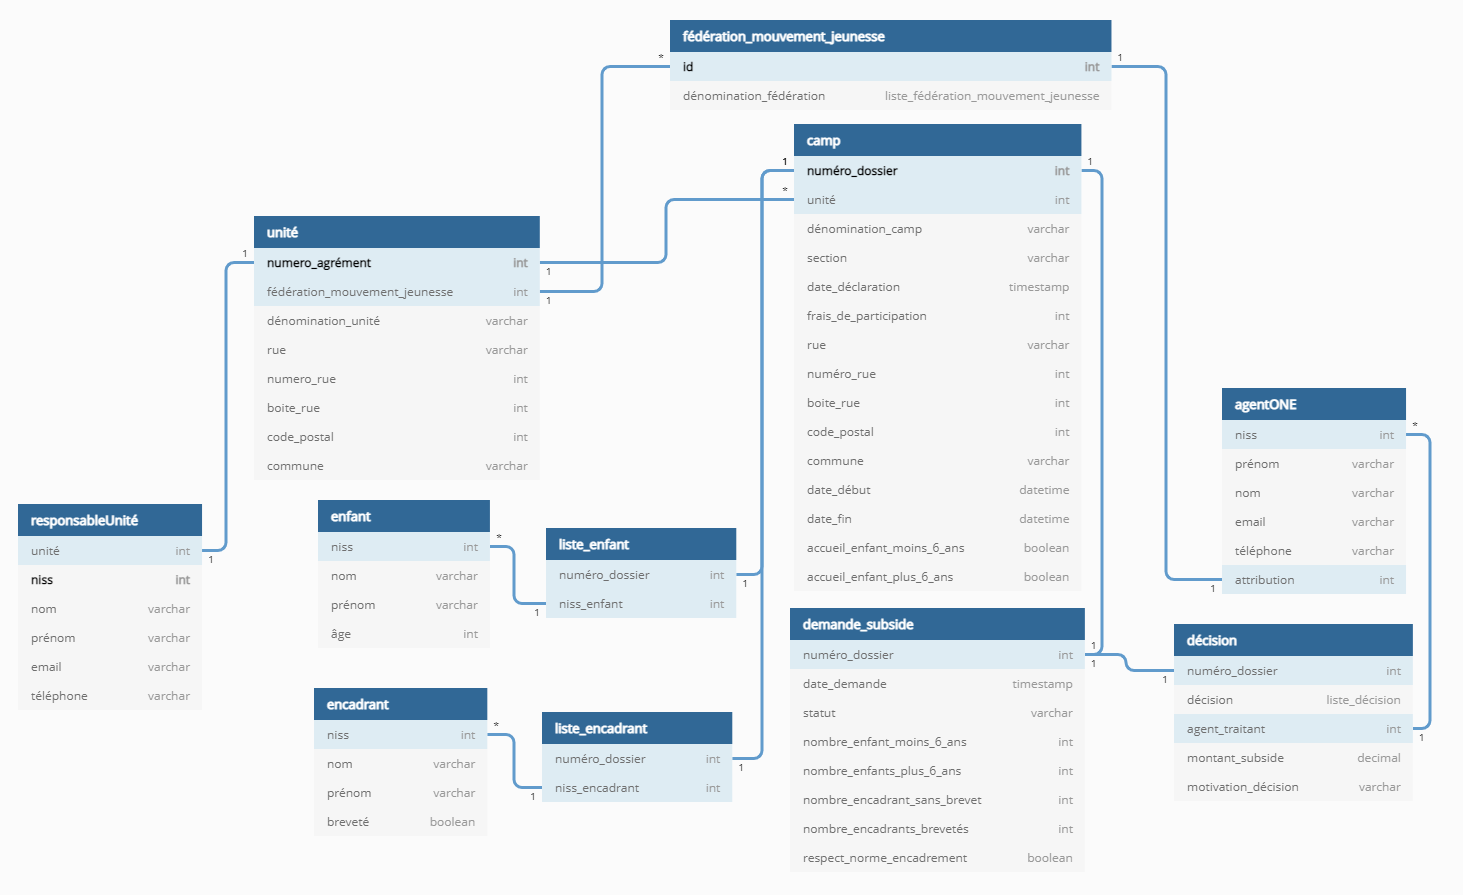
\includegraphics[width=17cm]{Pictures/modele_lr.png}
    \caption{Schéma logique relationnel}
    \label{fig:modele_lr}
\end{figure}


\section{Explication du schéma}
\subsection{Traduction de l'héritage}
Dans la mesure où les personnes ne peuvent avoir le rôle d'encadrants, d'enfants, de responsable d'unité ou agent ONE, qui correspond à une relation totale et exclusive, nous avons opté pour conserver les sous-entités. 

Chaque sous-entités reçoivent donc les attributs de la super-entité.


\subsection{Traduction de certaines associations et contraintes qui en découlent}
\subsubsection{Attribution des agents ONE: gestionnaire de dossiers}
Chaque agent ONE possède une attribution qui lui est propre. Cette attribution est liée à la fédération de mouvement de jeunesse dont il a la charge des dossiers.
\subsubsection{Résolution des cas de many to many pour les listes enfants et encadrants}
Les enfants et les encadrants peuvent participer à plusieurs camps durant une même année. Afin de prévoir ce cas de figure, deux tables viennent compléter le schéma afin d'établir des relations entre participants à de multiples camps. Un attribut année à également été ajouté afin de faciliter les manipulations de données.

\subsection{Choix de ne pas historiser le responsable d'unité}
Concernant la possibilité d'avoir un historique des responsables d'unité, il nous ne nous a pas jugé nécessaire d'ajouter cette dimension. Nous aurions pu résoudre ce cas en créant une entité "mandat" avec l'identité du responsable de projet et l'année concerné.

Seulement, l'ONE conserve les courriers officiels avec le destinataire et son adresse (archivage comptable). Nous saurions par ce biais qui s'occupait dès lors de l'envoie des déclarations et des demandes de subsides.

Cette informations aurait pu servir pour les unités (une base de données de ses membres et de ses mandataires à l'année), mais ne soulève pas un besoin dans notre cas d'application. En effet, si le responsable de projet venait à changer en cours d'année, il est plus utile d'envoyer et de contacter son successeur. 


%titre repris telle quelle des consignes

%---- Code de création de la base de données -----
\chapter{Code de création de la base de données}
\section{Script SQL (DDL) de création de la base de données}
\subsection{Création des tables: explications}
Le code infra permet de créer les tables et leurs attributs respectifs. Pour chaque table, les clefs primaires et étrangères ont été établies. Certaines contraintes ont été rejetées par PhpMyAdmin, mais pourront être gérées via le code php.

\subsection{Code de création des tables}
\inputminted[breaklines =true, autogobble, linenos, frame = single]{sql}{Codes/code_creation.tex}

\subsection{Code de création des clés étrangères}
\inputminted[breaklines =true, autogobble, linenos, frame = single]{sql}{Codes/code_key.tex}

Le résultat de ce script dans phpMyAdmin:voir figure \ref{fig:pmy_creation_fk}.

\subsection{Diagramme de relation entre les entités}
\begin{figure}[H]
    \centering
    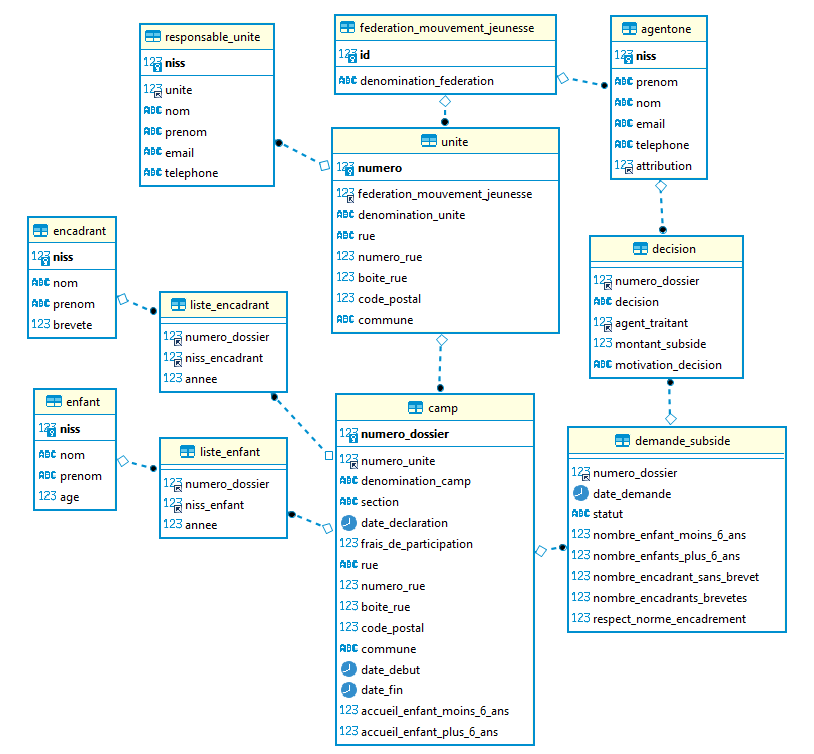
\includegraphics[width=17cm]{Pictures/er_diagram.png}
    \caption{Vue Dbeaver sur la base de données globale, avec relation entre les entités.}
    \label{fig:er_diagram}
\end{figure}



\section{Élément de SQL avancés}
\subsection{Prédicats: check des tables}
\subsubsection{Vérifications sur les dates de camps}
Un premier check permet de vérifier que la date de fin est bien cohérente avec la date de début.

%ajouter code 

Un deuxième permet de ne pas introduire de demande de subsides tant que le camp ne s'est pas terminé. 

%ajouter code


Concernant les dates calendrier (30 avril, 30 septembre) où la déclarations ou la demande de subsides doit être rentrées, elle se gérera au niveau du formulaire. 

Nous n'avons pas implémenté non plus le check sur les conflits de dates concernant les présences; une possibilité est d'ajouter des attributs de date dans la table liste\_enfant et liste\_encadrant.

\subsubsection{vérifications sur les âges}
Concernant les enfants et les encadrants, la première liste ne doit présenter que des enfants de moins de 15 ans, tandis que la seconde d'au moins 16 ans.



\subsection{Les vues}

\subsubsection{Vue pour les fédérations sur les unités fédérés}




\subsubsection{Vue uniquement sur les camps d'une unité précise}



\subsubsection{Vue sur les dossiers d'un agent (en fonction de sa fédération)}








\subsection{Les triggers}
\subsubsection{Attribution d'un dossier à un agent ONE}

\subsubsection{Calcul du nombre de participant lorsqu'une demande de subsides a été rentrée}




\subsection{droit d'accès}
\subsubsection{Agent ONE}
Accès à toutes les tables


\subsubsection{Responsable d'unité}
Accès uniquement à son unités: en modification camps déclarés, demandes de subsides. En consultation: décision de l'ONE. 



\subsubsection{Animateurs d'unité}
Accès uniquement en consultation à son unités et à ses camps. 






%\subsection{Contraintes de clefs primaires, uniques, externes}




\section{Script SQL (insert)}



%---- Application-web ------
\chapter{Application-web}
\section{Écran de consultation d'un des tables}



\section{Écran de consultation d'un élément d'une des tabkes}


\section{Écran permettant d'insérer un élément dans une tables}



\section{Écran affichant des informations agrégées}



%Bibliography
%\nocite{*}
%\printbibliography[type=article,title=Articles]

\end{document}